\documentclass[10pt]{article}

\usepackage[margin=1in]{geometry}
\usepackage{mathptmx}
\usepackage[T1]{fontenc}
\usepackage{listings}
\usepackage{xcolor}
\usepackage{hyperref}
\usepackage{graphicx}
\usepackage{float}
\usepackage{tikz}
\usetikzlibrary{arrows.meta,calc,positioning,shapes.geometric}

\lstdefinestyle{code}{
  basicstyle=\ttfamily\small,
  breaklines=true,
  frame=single,
  columns=fullflexible,
  showstringspaces=false
}

\title{Deadlock Detection Tool}
\author{James Widner\\KSU-ID: 001121770}
\date{May 4, 2026}

\begin{document}
\maketitle

\begin{abstract}
I built a small Go command-line program to test deadlock detection on a fixed resource-allocation snapshot. The program reads a JSON file, checks that the resource counts are valid, computes available instances, builds a wait-for graph, searches that graph for cycles, and prints a short recovery recommendation. I also added a simplified safe-state pass so the output can distinguish a real circular wait from a state where one process can still finish and release resources. The main result is practical rather than theoretical: for a known snapshot, deadlock detection is just finite graph analysis. The report also notes the boundary of that result. Predicting every possible future deadlock for arbitrary programs would require reasoning about future inputs, scheduling, and control flow, which connects the broader prediction problem to undecidability.
\end{abstract}

\section{Introduction}

Operating systems allow many programs to run at the same time. That is useful, but it also means programs can compete for limited resources such as files, printers, memory regions, database locks, network connections, and device handles. A deadlock can happen when one process keeps a resource while waiting for another resource, and that wait becomes part of a circular chain.

Deadlock matters because a deadlocked process cannot make progress by itself. In a real system this can cause an application to freeze, a server request to hang, or an entire subsystem to become unavailable. Because operating systems must manage shared resources, they need methods for detecting, avoiding, preventing, or recovering from deadlock.

For this project I kept the scope intentionally small. The tool does not inspect the real kernel or attach to live processes. Instead, I wrote a simulator that takes the kind of resource-allocation snapshot used in operating-systems examples and turns it into a wait-for graph. I chose this approach because it makes the output easy to check by hand: if the graph contains a cycle, the cycle itself explains which processes are stuck.

\section{Background Information and Motivation}

A deadlock can occur when four necessary conditions hold at the same time: mutual exclusion, hold and wait, no preemption, and circular wait \cite{osc}. In the examples for this project, the resources are treated as exclusive instances. For example, if \texttt{P1} holds the only printer and requests the only scanner, it cannot continue until the scanner is released.

Operating systems textbooks usually divide the responses into prevention, avoidance, detection, and recovery \cite{tanenbaum}. Prevention changes the rules so at least one necessary condition cannot occur. Avoidance, such as Banker's Algorithm, checks whether a grant would keep the system in a safe state. Detection allows the system to reach a bad state, but looks for it later and recovers by aborting, rolling back, or preempting a process.

This project focuses on detection because it is concrete enough to implement and test in a short program. Given a fixed set of processes, resources, allocations, and requests, the current state can be modeled as a finite graph. A graph cycle can be found with depth-first search, so the detection pass always terminates.

This is different from predicting every future deadlock in arbitrary programs. That broader question depends on inputs, branches, loops, and thread scheduling. A perfect predictor would need to answer questions about all possible executions of an arbitrary program, which is why the report connects the broader prediction problem to the Halting Problem \cite{turing}. The simulator is meant to keep those two claims separate: current-state detection is practical; perfect future prediction is not.

\section{Problem Definition}

The project solves the following practical problem:

\begin{quote}
Given a finite snapshot of processes, resources, current allocations, and current outstanding requests, determine whether the system is currently deadlocked. If deadlock exists, identify the cycle of processes and recommend recovery or prevention actions.
\end{quote}

The input is not program source code, and the output should not be read as a prediction about every future schedule. The program only answers the question represented by the JSON file it is given.

\section{Proposed Solution}

The solution is to represent the snapshot as a wait-for graph. Each node is a process. If process \(P_1\) is waiting for a resource currently held by process \(P_2\), the graph contains a directed edge from \(P_1\) to \(P_2\). A cycle means each process in that cycle is waiting on another process in the same group, so none of them can make progress without outside intervention.

For example, suppose the system has three processes:

\begin{itemize}
  \item \(P_1\) holds the printer and requests the scanner.
  \item \(P_2\) holds the scanner and requests the database.
  \item \(P_3\) holds the database and requests the printer.
\end{itemize}

The wait-for graph is:

\[
P_1 \rightarrow P_2 \rightarrow P_3 \rightarrow P_1
\]

This cycle proves that the system is deadlocked.

\begin{figure}[H]
\centering
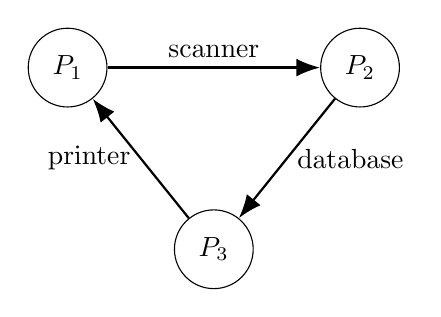
\begin{tikzpicture}[
  node distance=2.7cm,
  process/.style={circle,draw,minimum size=1cm,font=\bfseries},
  edge/.style={-{Latex[length=3mm]},thick}
]
  \node[process] (p1) {$P_1$};
  \node[process,right=of p1] (p2) {$P_2$};
  \node[process,below=1.8cm of $(p1)!0.5!(p2)$] (p3) {$P_3$};
  \draw[edge] (p1) -- node[above]{scanner} (p2);
  \draw[edge] (p2) -- node[right]{database} (p3);
  \draw[edge] (p3) -- node[left]{printer} (p1);
\end{tikzpicture}
\caption{Wait-for graph for the sample deadlock. Each arrow points from a waiting process to the process holding the needed resource.}
\end{figure}

\section{Methods}

The implementation follows six main steps. I kept these steps separate in the code because it made the command output easier to debug: when a result looked wrong, I could compare the available-resource table, then the wait-for edges, then the cycle result.

\begin{figure}[H]
\centering
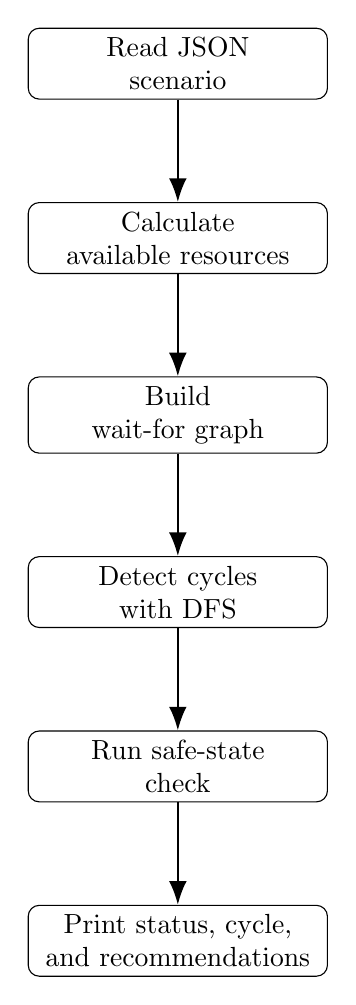
\begin{tikzpicture}[
  node distance=1.3cm,
  flowstep/.style={rectangle,draw,rounded corners,align=center,minimum width=3.8cm,minimum height=0.8cm},
  arrow/.style={-{Latex[length=3mm]},thick}
]
  \node[flowstep] (input) {Read JSON\\scenario};
  \node[flowstep,below=of input] (available) {Calculate\\available resources};
  \node[flowstep,below=of available] (graph) {Build\\wait-for graph};
  \node[flowstep,below=of graph] (cycle) {Detect cycles\\with DFS};
  \node[flowstep,below=of cycle] (safe) {Run safe-state\\check};
  \node[flowstep,below=of safe] (output) {Print status, cycle,\\and recommendations};

  \draw[arrow] (input) -- (available);
  \draw[arrow] (available) -- (graph);
  \draw[arrow] (graph) -- (cycle);
  \draw[arrow] (cycle) -- (safe);
  \draw[arrow] (safe) -- (output);
\end{tikzpicture}
\caption{Analysis workflow used by the deadlock detection tool.}
\end{figure}

\subsection{Input Parsing}

The program reads a JSON file with three maps: total resources, current allocations, and current requests. Allocation and request keys use the format \texttt{process:resource}. I first considered a more nested JSON structure, but the flat key format made the example files shorter and easier to type from the command line. The tradeoff is that the loader has to validate the key format carefully.

\begin{lstlisting}[style=code,caption={Example deadlock scenario}]
{
  "resources": {
    "printer": 1,
    "scanner": 1,
    "database": 1
  },
  "allocations": {
    "P1:printer": 1,
    "P2:scanner": 1,
    "P3:database": 1
  },
  "requests": {
    "P1:scanner": 1,
    "P2:database": 1,
    "P3:printer": 1
  }
}
\end{lstlisting}

\subsection{Validation}

The tool validates the scenario before detection. It checks that resource totals are not negative, allocation and request amounts are not negative, all referenced resources exist, and no resource is over-allocated. I added this after testing an invalid input where a process held two instances of a resource that only had one total instance. Without validation, the graph pass could still run, but the result would describe an impossible system state.

\subsection{Available Resource Calculation}

For each resource, the tool subtracts allocated instances from the total number of instances:

\[
Available(R) = Total(R) - \sum Allocated(P, R)
\]

This determines whether a pending request can be satisfied immediately or whether it must wait for another process to release the resource.

\subsection{Wait-For Graph Construction}

For every request that cannot be satisfied with currently available resources, the tool finds processes that hold the requested resource. If process \(P_i\) requests resource \(R\), and process \(P_j\) currently holds \(R\), the tool adds the edge:

\[
P_i \rightarrow P_j
\]

Multiple resources can create the same wait relationship, so the implementation removes duplicate edges before printing. It also sorts process and resource names to keep the output stable between runs; otherwise Go's randomized map iteration can make screenshots and tests change order.

\subsection{Cycle Detection}

The program uses depth-first search to find cycles in the wait-for graph. During traversal, each process is marked as unvisited, currently visiting, or completed. If the search reaches a process that is already in the current recursion stack, a cycle has been found. I store the stack index for each active process so the program can print the actual cycle instead of only returning a boolean.

\subsection{Safe-State Check}

The tool also performs a safe-state check inspired by Banker's Algorithm. It repeatedly looks for a process whose current outstanding requests can be satisfied by the available resources. If such a process can finish, the tool releases its allocated resources into the available pool and continues. If all processes can finish, the state is safe. If some processes cannot finish, the state is unsafe.

This safe-state result is not the same as the cycle result. In this project it is mainly a second explanation for the user: the wait-for graph says whether there is a current circular wait, while the safe-state pass shows whether there is at least one order in which every process can complete.

\section{Implementation and Experimental Results}

The project is implemented in Go. The command-line entry point is located in \texttt{cmd/deadlock}. The core detection logic is located in \texttt{internal/deadlock}. The examples are located in \texttt{examples}. I kept the detector in an \texttt{internal} package so the command-line formatting code would not be mixed with the graph and validation logic.

The project can be run with:

\begin{lstlisting}[style=code]
go run ./cmd/deadlock -file examples/deadlock.json
\end{lstlisting}

The test suite can be run with:

\begin{lstlisting}[style=code]
go test ./...
\end{lstlisting}

\subsection{Experiment 1: Deadlocked System}

The first experiment uses three resources and three processes. Each process holds one resource and requests the next resource in a cycle. The output is:

\begin{figure}[H]
\centering
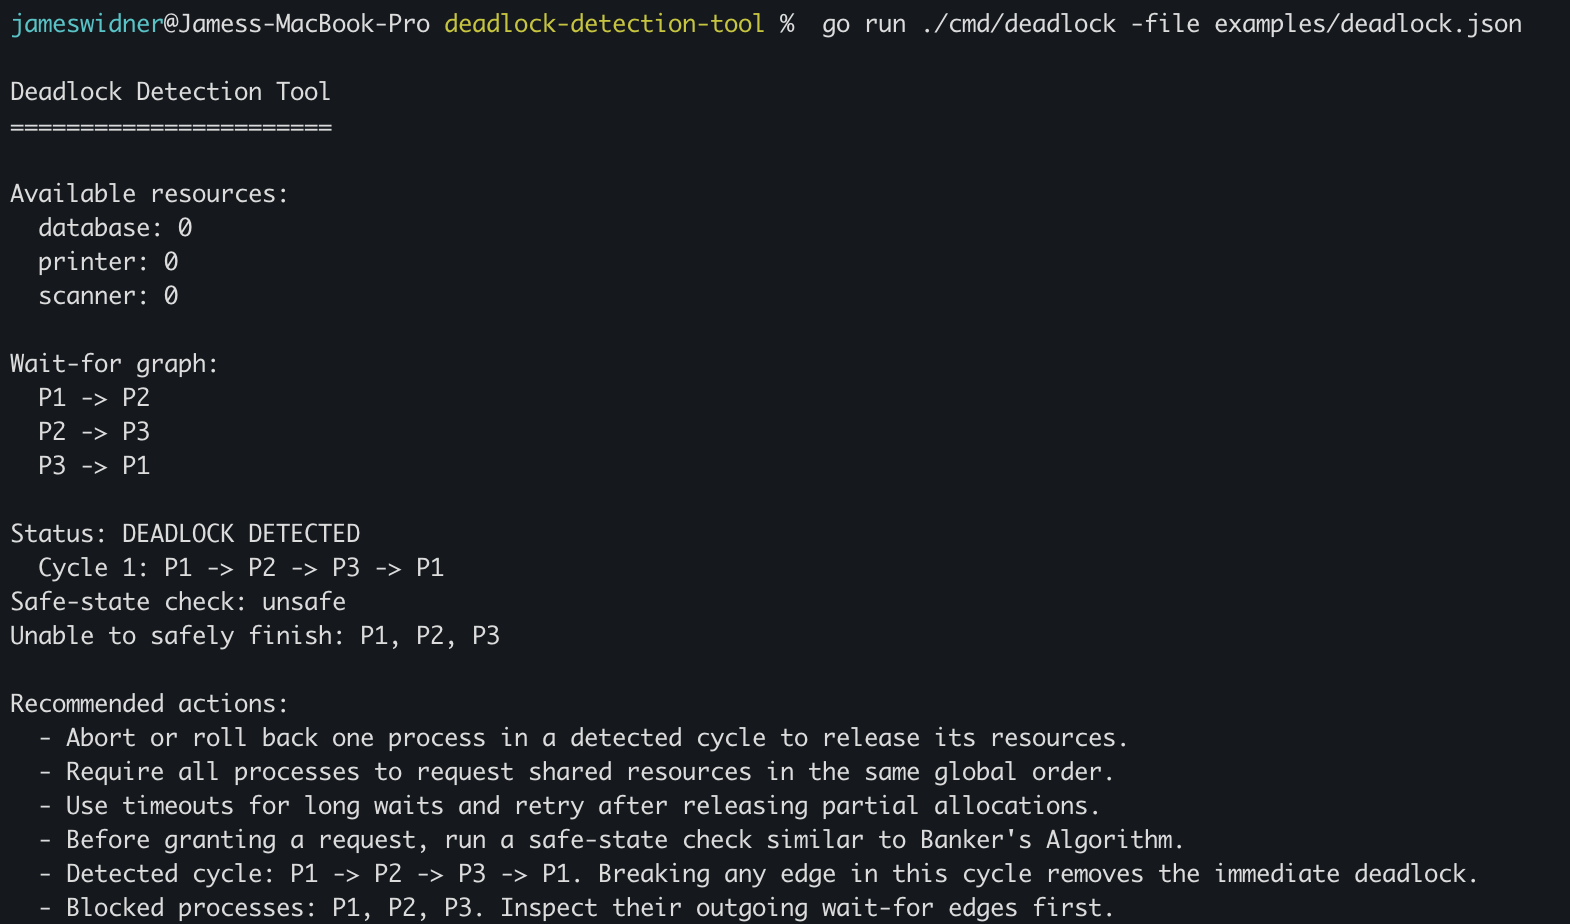
\includegraphics[width=\textwidth]{figures/deadlock-terminal-screenshot.png}
\caption{Terminal screenshot from running \texttt{go run ./cmd/deadlock -file examples/deadlock.json}. The tool detects the cycle \texttt{P1 -> P2 -> P3 -> P1} and reports an unsafe state.}
\end{figure}

In this run, all three resources have zero availability after the initial allocations. The printed wait-for edges are \texttt{P1 -> P2}, \texttt{P2 -> P3}, and \texttt{P3 -> P1}. That matches the scenario file and confirms that the cycle detector is finding the circular wait rather than just reporting that resources are unavailable.

\subsection{Experiment 2: Safe System}

The second experiment includes enough available resources for the system to make progress. The output is:

\begin{figure}[H]
\centering
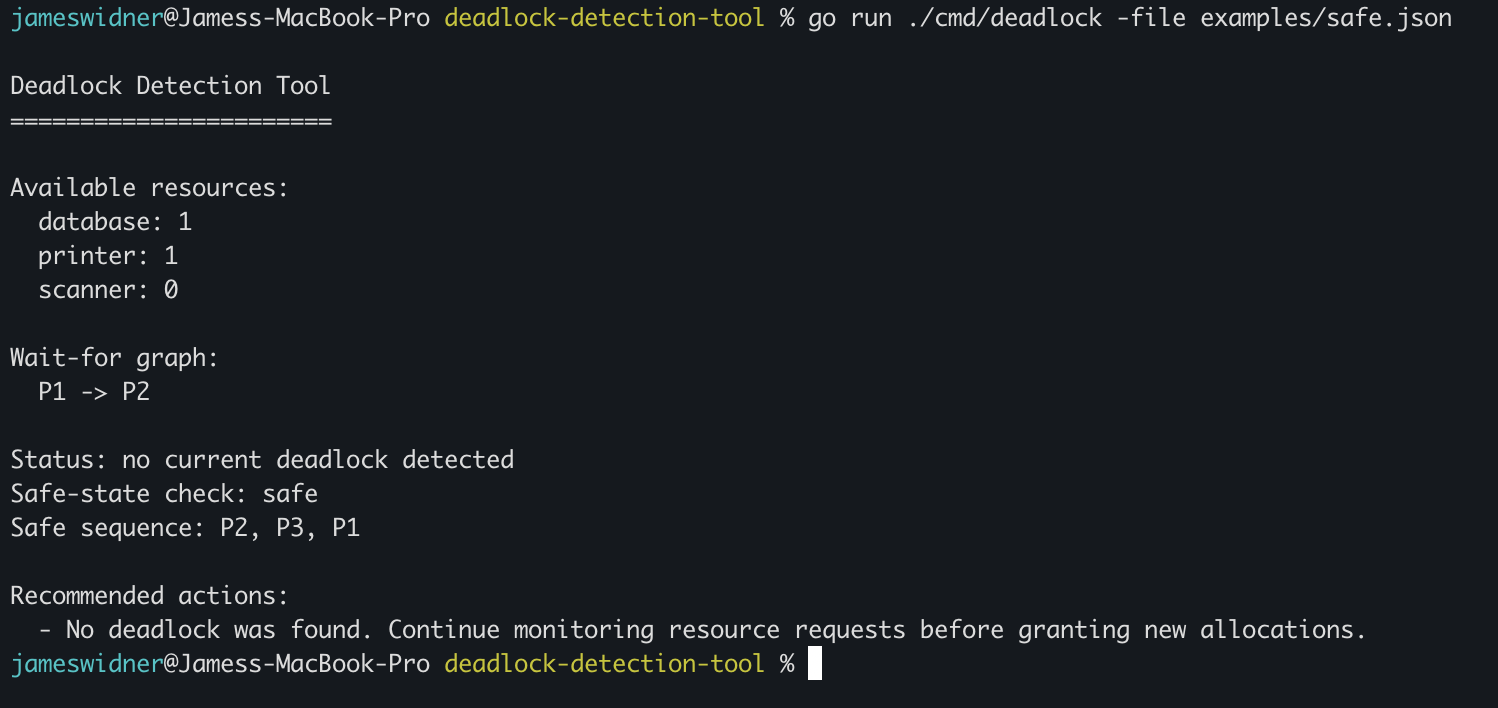
\includegraphics[width=\textwidth]{figures/safe-terminal-screenshot.png}
\caption{Terminal screenshot from running \texttt{go run ./cmd/deadlock -file examples/safe.json}. The tool reports no current deadlock and gives the safe sequence \texttt{P2, P3, P1}.}
\end{figure}

This run was useful because it caught an early assumption I almost made: waiting does not automatically mean deadlock. Process \(P_1\) is waiting for \(P_2\), but \(P_2\)'s request can be satisfied, so \(P_2\) can finish and release its resources. The reported safe sequence, \texttt{P2, P3, P1}, is one valid completion order for this snapshot.

\subsection{Testing}

The project includes automated unit tests. The tests check three cases that were easy to get wrong while writing the detector: a two-process cycle, a safe state that still has a waiting edge, and an invalid over-allocation. The over-allocation test is especially important because the rest of the analysis assumes the snapshot is physically possible.

\section{Discussion}

The graph-based design is useful because it explains the reason for the deadlock. A simple status message such as ``deadlocked'' is not enough for recovery. The output needs to identify the process group involved, because aborting an unrelated process would not release the resource chain that matters.

The recommendations printed by the tool are deliberately simple. Aborting or rolling back one process in a cycle is a recovery method. Requiring a global resource order is a prevention method. Checking safe states before granting requests is an avoidance method. Timeouts are included because they are a practical engineering response, even though they do not prove the absence of deadlock.

The project also helped clarify the difference between detection and prediction. Deadlock detection for the current snapshot is decidable because the graph is finite and the DFS has a fixed amount of work. Predicting whether an arbitrary program will ever reach a deadlock is a different question. A program may depend on unknown input, nondeterministic scheduling, or loops that may or may not terminate. That is why I treated the Halting Problem as background for the limitation, not as something the tool itself tries to solve.

\section{Limitations}

The main limitation is that the tool analyzes a snapshot rather than a live operating system. It does not inspect actual kernel locks, actual file descriptors, or real process scheduling. The input scenario must be written manually in JSON, so the quality of the result depends on whether the JSON accurately describes the system state.

Another limitation is that the safe-state check is simplified. Full Banker's Algorithm usually requires maximum claims for each process \cite{osc}. This simulator uses current outstanding requests and current allocations, which is enough for the examples in this project but does not cover every full avoidance scenario.

The tool also does not decide which process should be aborted. It recommends breaking a cycle, but a real operating system would also consider priority, amount of work lost, user impact, and whether a process can safely roll back. Adding a cost model for that decision would be a reasonable extension.

\section{Conclusion}

This project demonstrates a practical deadlock detection method for a known operating-system resource snapshot. By modeling processes and resources as a wait-for graph, the tool can detect cycles and identify the exact processes involved in a current deadlock. The safe-state check and recommendation output add context, but the core result is the cycle in the wait-for graph.

The main lesson from the implementation is the distinction between a finite current-state problem and a general future-prediction problem. The first can be solved with ordinary graph analysis. The second is limited by the same kind of undecidability issue that appears when reasoning about arbitrary program behavior.

\begin{thebibliography}{9}

\bibitem{osc}
Abraham Silberschatz, Peter Baer Galvin, and Greg Gagne.
\textit{Operating System Concepts}.
10th ed., Wiley, 2018.

\bibitem{tanenbaum}
Andrew S. Tanenbaum and Herbert Bos.
\textit{Modern Operating Systems}.
4th ed., Pearson, 2015.

\bibitem{dijkstra}
Edsger W. Dijkstra.
Cooperating Sequential Processes.
In \textit{Programming Languages}, Academic Press, 1968.

\bibitem{turing}
Alan M. Turing.
On Computable Numbers, with an Application to the Entscheidungsproblem.
\textit{Proceedings of the London Mathematical Society}, Series 2, Vol. 42, 1936.

\end{thebibliography}

\end{document}
